\documentclass[10pt]{article}
\usepackage{lipsum}
\usepackage{indentfirst}
\usepackage[portuguese]{babel}
\usepackage{graphicx}
 \usepackage{siunitx}
\usepackage[a4paper,left=2cm,right=2cm,top=2cm,bottom=2cm]{geometry}

\linespread{1.5}
\begin{document}
	

\title{\uppercase{\textbf{Relatório: Estudo térmico de gases e sólido}}}
\author{Saulo Ferreira de Souza 83339 \protect\\ Rodrigo Otavio de Lima 89386}
\maketitle

\setlength{\parindent}{2cm}

\section{OBJETIVOS}

Detalhar as metodologias e procedimentos utilizados no estudo térmico de gases e sólido, utilizando gráficos e tabelas como ferramentas auxiliares.

\section{INTRODUÇÃO}

Ao longo do dia é muito comum observarmos o movimento de queda de objetos. Seja uma caneta que cai da mesa, um pingo de chuva que cai na terra ou mesmo uma folha seca que cai da árvore no inverno. Dessa forma, o estudo desse tipo de movimento se torna algo importante para o  entendimento  de  processo tais  como os  exemplificados.  Normalmente,  num  movimento  de queda  como  esses,  a  força  de  atrito  também  influencia  no  movimento;  entretanto,  num  tratamento mais simplificado, desconsiderando os efeitos desta força, pode-se dizer que a força peso é a responsável pela queda do objeto até o chão. 

Nesta prática, foi realizado um estudo comparativo entre o movimento parabólico de um projétil lançado  horizontalmente  e o movimento de  um corpo em queda livre  (ou seja, sem velocidade horizontal).

Chama-se lançamento horizontal quando um corpo é lançado de uma certa altura com velocidade inicial horizontal diferente de  zero, conforme  a  Figura 1. O  movimento de  uma  bola  caindo de 
uma mesa é descrito por esse tipo de lançamento.

\begin{figure}
	\begin{center}
		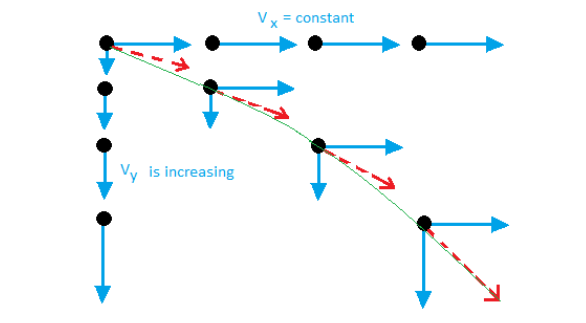
\includegraphics[scale=0.5]{movimento_horizontal.png}
		\caption{Lançamento horizontal de um projétil, com velocidade constante e sob efeito apenas da força da gravidade}
		\label{fig:horizontal}
	\end{center}
\end{figure}

Desconsiderando as forças de dissipação, temos que o projétil está sujeito à força gravitacional que, num sistema de coordenadas cartesiana usual, é vertical para baixo. Portanto, a componente vertical do vetor velocidade ($v_y$) é variável, pois nesta direção atua a aceleração da gravidade ($g$), sempre para baixo, oriunda da força gravitacional. Já a componente horizontal do vetor velocidade ($v_y$) é constante, pois nenhuma força (desprezando qualquer tipo de resistência) atua sobre o corpo nessa direção.

Assim, as equações para cada componente, adotando o eixo vertical ($y$) positivo orientado para baixo, são:

\begin{equation}
\vec{r} = \vec{r}_0 + \vec{v}_0t + \frac{1}{2}\vec{a}t^2
\label{eq:posicao}
\end{equation}

Como na horizontal $a_x=0$ e na vertical $a_y=g$, teremos:

\begin{equation}
x = x_0 + v_{0x}t
\label{eq:posicao_horizontal}
\end{equation}

\begin{equation}
y = y_0 + v_{0y}t + \frac{1}{2}gt^2
\label{eq:posicao_vertical}
\end{equation}

Note que, se $v_{0x}$ for nulo, o movimento na vertical será o que chamaremos de ``queda livre'', a queda simples de um objeto sem velocidade horizontal. Nesta prática, portanto, foram estudados os dois movimentos: o lançamento horizontal ($v_{0y} = 0$) e queda livre.

\section{METODOLOGIA}

\subsection{MATERIAL UTILIZADO}

Para a prática de expansão térmica de metais, utilizamos tubos metálicos, gerador de vapor, termômetro, suporte para medida de variação de tamanho dos tubos.
Para a prática de gases ideais, utilizamos uma montagem igual a ilustrada na figura \ref{fig:aparato_gases_ideais}, contendo os seguintes itens: Reservatório de gás, manômetro de mercúrio, régua, reservatório de água com termostato e circulador de água e termômetros. Para os gráficos, foi utilizado papel monolog. 

\begin{figure}
	\begin{center}
		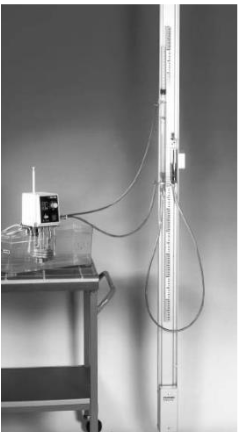
\includegraphics[scale=0.5]{aparato_gases_ideais.png}
		\caption{Esquema do experimento}
		\label{fig:aparato_gases_ideais}
	\end{center}
\end{figure}

Para esta montagem, o volume do reservatório onde o gás está contido é dado em mililitros ($ml$) e é determinado pela altura $a$ que corresponde ao nível superior da borda da coluna de mercúrio, mais um volume de $1,01ml$ referente a parte superior do reservatório (parte laranja). Assim, o valor do volume deve ser dado por:

\begin{equation}
	V = (0,1021)a + 1,01
	\label{eq:volume_gases_ideais}
\end{equation}

A pressão é medida em $kPa$ e o valor pode ser determinado por

\begin{equation}
P_{gas} = 94,06 + 0,1333h
\label{eq:pressao_gases_ideais}
\end{equation}

onde o valor $94,06$ corresponde a pressão atmosférica em Viçosa e $0,1333$ ao produto $pg$.

A temperatura, medida em graus Celsius foi transformada em Kelvin seguindo a relação:

\begin{equation}
T(K) = T(ºC) + 273,15
\label{eq:celsius_kelvin}
\end{equation}

\subsection{PROCEDIMENTO}

\subsubsection{Expansão Térmica}
Na montagem utilizada (figura \ref{fig:aparato_expansao_termica}), um tubo metálico tem uma extremidade fixa e outra livre cujo avanço foi medido indiretamente através do deslocamento angular de um eixo.

A temperatura ambiente foi medida utilizando um termômetro de mercúrio, encontrando o valor de $(21,00 \pm 0,05) ºC$. Foram utilizados 3 tubos (Alumínio, Latão e Cobre), e seus comprimentos foram medidos em temperatura ambiente utilizando uma fita métrica milimetrada, encontrando os valores de $(75,00 \pm 0,05)cm$, $(74,80 \pm 0,05) cm$ e $(74,80 \pm 0,05)cm$ respectivamente. Nos experimentos com cada tubo, o ângulo inicial do mostrador foi iniciado a partir de $0$. A temperatura do vapor na saída da mangueira conectada ao gerador de vapor ($T_c$) foi medida utilizando o termômetro de mercúrio, com o valor de $(95,00 \pm 0,05)ºC$.

A base horizontal da calha foi nivelada utilizando o nível para garantir que a esfera possuísse $v_{0y} = 0$ ao abandonar-la, garantindo um lançamento horizontal.

\begin{figure}
	\begin{center}
		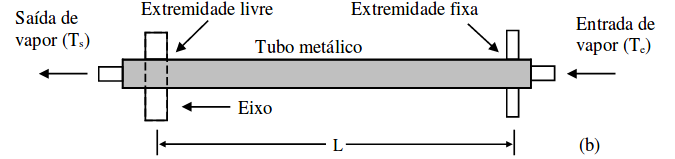
\includegraphics[scale=0.5]{aparato_expansao_termica.png}
		\caption{Esquema do experimento}
		\label{fig:aparato_expansao_termica}
	\end{center}
\end{figure}

Para obter o valor de $x$, o prumo e a fita adesiva foram utilizados para marcar no piso o ponto $x_0$, ficando alinhado com o ponto \textbf{B}. A folha de papel carbono coberta com papel branco foi utilizada para definir o local onde a esfera atingiu o piso, definindo o ponto \textbf{C}. Desta forma, foi utilizada a régua centimetrada para medir a distância do ponto $x_0$ ao ponto \textbf{C}, definindo o valor de $x$ em cada repetição do experimento. O valor de $x$ encontrado em cada repetição do experimento para cada altura $y$ pode ser encontrado na Tabela \ref{tab:table_1}


\begin{table}[h!]
	\begin{center}
		\resizebox{\textwidth}{!}{	
		\begin{tabular}{|c|c|c|c|c|c|c|c|c|}
			\hline
			$y (cm)$ & 138 & 128 & 118 & 108 & 98 & 88 & 78 & 68 \\
			\hline
			$x_1 (cm)$ & 105 & 98 & 93,6 & 88,8 & 83 & 79,6 & 74,3 & 70\\
			\hline		
    		$x_2 (cm)$ & 110 & 98,1 & 94,3 & 89,1 & 83,4 & 80 & 74,5 & 70,4 \\
			\hline	
			$x_3 (cm)$ & 120 & 99 & 94,5 & 89,8 & 83,7 & 80 & 74,9 & 71,2\\
			\hline	
			$\overline{x} \pm \Delta x (cm) $ & $111,67 \pm 5,56$ & $98,37 \pm 0,42$ & $94,13 \pm 0,36$ & $89,23 \pm 0,38$ & $83,36 \pm 0,25$ & $79,85 \pm 0,18$ & $74,57 \pm 0,22$ & $70,53 \pm 0,44$\\
			\hline	
			$x^2 \pm \Delta x^2 (cm^2) $ & $12508,3 \pm 1261,11$ & $9676,2 \pm 83,2$ & $8861,23 \pm 66,85$ & $7962,76 \pm 67,52$ & $6950,08 \pm 40,72$ & $6378,72 \pm 28,37$ & $5560,25 \pm 33,17$ & $4975,2 \pm 62,83$\\ 
			\hline	
		\end{tabular}}
		\caption{Resultados obtidos em cada repetição do experimento}
		\label{tab:table_1}
	\end{center}
\end{table}

A velocidade inicial de lançamento ($v_{0x (esperado)}$) foi obtida através da conservação de energia (\ref{eq:conservacao}), com $g = (9,78 \pm 0,05) ms^2$, $h = (0,45 \pm 0,0005)m$ e momento de inércia da esfera $I = \frac{2MR^2}{5}$


\begin{equation}
Mgh = \frac{1}{2}Mv_{0x}^2 \times \frac{1}{2}I\omega^2 \Rightarrow
Mgh = \frac{1}{2}Mv_{0x}^2 \times \frac{1}{2} \times \frac{2MR^2}{5}  \times \frac{v_{0x}^2}{R^2} \Rightarrow
v_{0x} = \sqrt{\frac{10}{7}gh} \Rightarrow v_{0x} = 2,51 m/s^2
\label{eq:conservacao}
\end{equation}

\subsubsection{Queda livre}

Para a queda livre, foram utilizadas duas esferas de massa  $27,6g$ e $16g$, obtidas utilizando uma balança, e diâmetros $18,8mm$ e $15,7mm$ respectivamente, obtidos utilizando o paquímetro. O tempo de queda livre das duas esferas foi calculado utilizando o equipamento da figura \ref{fig:queda_livre}. Para tal, as esferas foram abandonadas de 8 alturas distintas. Para medir as alturas, foi utilizada uma régua centimetrada. As Tabelas \ref{tab:primeira_esfera} e \ref{tab:segunda_esfera} mostram os valores coletados no experimento para cada esfera.

\begin{figure}
	\begin{center}
		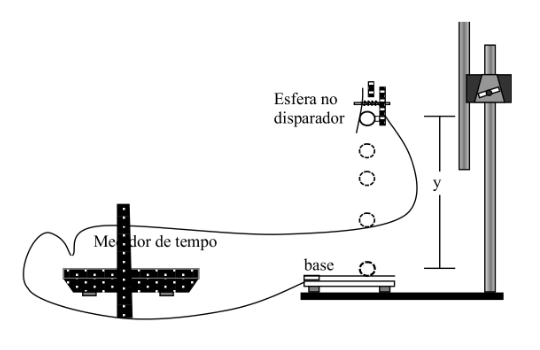
\includegraphics[scale=0.5]{queda_livre.png}
		\caption{Equipamento para cálculo do tempo de queda livre de uma esfera}
		\label{fig:queda_livre}
	\end{center}
\end{figure}

\begin{table}[h!]
	\begin{center}
		\resizebox{\textwidth}{!}{	
			\begin{tabular}{|c|c|c|c|c|c|c|c|c|}
				\hline
				$y (m)$ & 1,80 & 1,60 & 1,40 & 1,20 & 1,00 & 0,80 & 0,60 & 0,40 \\				
				\hline
				$t_1(s)$ & 0,6110 & 0,579 & 0,539 & 0,497 & 0,456 & 0,423 & 0,357 & 0,287\\
				\hline	
				$t_2(s)$ & 0,610 & 0,578 & 0,540 & 0,497 & 0,453 & 0,423 & 0,353 & 0,289\\
				\hline
				$t_{med} \pm \Delta t_{med} (s) $ & $0,6105 \pm 0,0005$ & $0,5785\pm 0,0005$ & $0,5395\pm 0,0005$ & $0,497$ & $0,4545\pm 0,0015$ & $0,423$ & $0,355\pm 0,002$ & $0,288\pm 0,001$\\
				\hline	
				$t_{med}^2 \pm \Delta t_{med}^2 (s^2) $ & $0,3727 \pm 0,0006$ & $0,3347\pm 0,0006$ & $0,2910\pm 0,0005$ & $0,2470$ & $0,2066\pm 0,0014$ & $0,1789$ & $0,1260\pm 0,0014$ & $0,0829\pm 0,0006$\\
				\hline	
		\end{tabular}}
		\caption{Dados coletados e calculados relativos à queda da esfera de $15,7mm$ }
		\label{tab:primeira_esfera}
	\end{center}
\end{table}

\begin{table}[h!]
	\begin{center}
		\resizebox{\textwidth}{!}{	
			\begin{tabular}{|c|c|c|c|c|c|c|c|c|}
				\hline
				$y (m)$ & 1,80 & 1,60 & 1,40 & 1,20 & 1,00 & 0,80 & 0,60 & 0,40 \\				
				\hline	
				$t_1(s)$ & 0,604 & 0,567 & 0,532 & 0,492 & 0,450 & 0,402 & 0,348 & 0,287\\
				\hline	
				$t_2(s)$ & 0,605 & 0,569 & 0,531 & 0,493 & 0,449 & 0,403 & 0,347 & 0,284\\
				\hline
				$t_{med} \pm \Delta t_{med} (s) $ & $0,6045 \pm 0,0005$ & $0,5680\pm 0,001$ & $0,5315\pm 0,0005$ & $0,4925\pm 0,0005$ & $0,4490\pm 0,0005$ & $0,4025\pm 0,0005$ & $0,3475\pm 0,0005$ & $0,2855\pm 0,0015$\\
				\hline	
				$t_{med}^2 \pm \Delta t_{med}^2 (s^2) $ & $0,3654 \pm 0,0006$ & $0,3226\pm 0,001$ & $0,2825\pm 0,0005$ & $0,2425\pm 0,0005$ & $0,2020\pm 0,0004$ & $0,1620\pm 0,0004$ & $0,1207\pm 0,0003$ & $0,0815\pm 0,0008$\\
				\hline	
		\end{tabular}}
		\caption{Dados coletados e calculados relativos à queda da esfera de $18,8mm$ }
		\label{tab:segunda_esfera}
	\end{center}
\end{table}

\section{RESULTADOS}

Os dados coletados em ambos experimentos foram utilizados na produção dos gráficos em papel milimetrado, anexados ao relatório. Para o lançamento horizontal, foi produzido um gráfico de altura por alcance, em seguida este gráfico foi linearizado elevando o alcance ao quadrado. A interseção com o eixo $y$ neste gráfico, representa a altura mínima de lançamento no experimento. Já a inclinação da reta representa a velocidade horizontal do lançamento ($v_{0x}$), que é constante. 

Para o experimento de queda livre, foi produzido um gráfico de altura por tempo, e foi linearizado elevando o tempo do quadrado. A interseção da reta com o eixo vertical não possui significado físico, já o coeficiente angular representa a gravidade, que é constate.

Da equação \ref{eq:posicao_vertical}, obtém-se a equação \ref{eq:vertical_simples}:

\begin{equation}
\Delta y = \frac{1}{2}g\Delta t^2 \Rightarrow g = 2\frac{\Delta y}{\Delta t^2}
\label{eq:vertical_simples}
\end{equation}

Aplicando os valores do gráfico linearizado para a esfera menor na equação \ref{eq:vertical_simples}, obtém se o seguinte valor para $g$:

\begin{equation}
g = 2\frac{(0,55-0,35)}{(0,1215-0,081)} \Rightarrow g = 9,88m/s^2
\label{eq:aceleracao_esfera1}
\end{equation}

Para o gráfico linearizado da esfera maior, obtém se o seguinte valor para $g$:
\begin{equation}
g = 2\frac{(0,6-0,4)}{(0,1215-0,081)} \Rightarrow g = 9,88m/s^2
\label{eq:aceleracao_esfera2}
\end{equation}

O erro relativo percentual é representado abaixo:

\begin{equation}
|\frac{9,78-9,88}{9,88}| \times 100 = 1,01\%
\end{equation}
\begin{equation}
\label{key}
\end{equation}

Como a área da superfície das esferas são diferentes, há uma diferença no tempo devido o atrito com o ar. Por conta disso, a aceleração será diferente, já que o somatório das forças diferem.

\section{CONCLUSÃO}

Os resultados encontrados nos experimentos foram de acordo com o esperado pela formulação teórica, com pequenos desvios aceitáveis. É possível notar que o experimento se aproximou dos valores teóricos, devido à suas repetições, confirmando a evidência de quanto mais se repete os testes experimentais, mais a média dos resultados observados converge para o valor esperado.  


\begin{thebibliography}{9}
	
	\bibitem{lamport94}
	``PRÁTICA: QUEDA LIVRE E LANÇAMENTO HORIZONTAL.''
	\textit{Departamento de Física, UFV.}


\end{thebibliography}

\end{document}

